% %!TEX root main.tex
\section{Introduction}
\label{sec:introduction}

A \emph{univariate formal series} over the rationals is a function $\N \to \Q$
(sometimes written $\powerseries \Q x$).
%
They arise in a variety of disciplines, \eg,
Taylor series in mathematical analysis~\cite{Rudin:Analysis:1976},
generating functions in combinatorics~\cite{Stanley:1986,Wilf:generatingfunctionology:2005},
and Z-transforms in engineering~\cite{OppenheimSchafer:DSP:1975}.
%
The denomination ``formal'' highlights the algebraic aspect, rather than the analytic one;
%which is convenient for the development of their theory;
for brevity, we will refer to formal series simply as series.

The theory of univariate series can be developed in several directions.
%
One direction is more popular in mathematics,
and considers \emph{multivariate series in commuting indeterminates $X = \set{x_1, \dots, x_d}$},
which are functions of the form $\N^d \to \Q$ for some $d \in \N_{\geq 1}$
(sometimes written $\powerseries \Q X$)~\cite{PemantleWilsonMelczer:CUP:2024}.
%
Another direction is more popular in theoretical computer science,
and considers \emph{multivariate series in noncommuting indeterminates $\Sigma = \set{a_1, \dots, a_d}$},
which are functions of the form $\Sigma^* \to \Q$
(sometimes called \emph{weighted languages} and written $\series \Q \Sigma$)~\cite{BerstelReutenauer:CUP:2010}.
%
In fact, noncommuting indeterminates are more general,
since we can recover commuting indeterminates as a special case:
%
Namely, as those series $f \in \series \Q \Sigma$ which are \emph{commutative},
\ie, $f(u) = f(v)$ for all words $u, v \in \Sigma^*$ which are permutations of each other.
%
This is the unifying view that we shall adopt.

In the context of formal languages and automata theory,
series in noncommuting indeterminates have been introduced by Schützenberger,
who considered the class of \emph{rational series}~\cite{Schutzenberger:IC:1961}
(\cf~\cite{BerstelReutenauer:CUP:2010} for an extensive introduction).
%
This class has since appeared in various areas of computer science and mathematics~\cite{HandbookWA},
such as speech recognition~\cite{MohriPereira:Riley:CSL:2002},
digital image compression~\cite[Part IV]{HandbookWA},
learning~\cite{BalleMohri:AI:2015},
quantum computing~\cite{BlondelJeandelKoiranPortier:SIAM:JoC:2005},
as well as in Bell and Smertnig's resolution~\cite{BellSmertnig:SM:2021}
of a conjecture of Reutenauer~\cite{Reutenauer:FCT:1979}.

Series have also been applied to control theory,
as put forward by the pioneering work of Fliess~\cite{Fliess:1981}.
%
Namely, he associated to a control system its \emph{characteristic series},
in such a way that the behaviour of the system as an input-output transformer
is uniquely determined by it~\cite[Lemme II.1]{Fliess:1981}.
%
He then recovered the rational series
as the characteristic series of the so-called \emph{bilinear systems}~\cite{Fliess:MST:1976}.
%
This is an extensively studied class~\cite{DAlessandroIsidoriRuberti:SIAMJoC:1974},
whose theory can be derived from well-known results for rational series
(\eg, decidability of equivalence checking and existence of minimal realisations).
%
It is in relation with control theory
that commutativity naturally enters the picture.
%
Fliess isolated an important subclass of bilinear systems,
namely those 
%, which we could call \emph{memoryless}
where the output at time $t$ depends only on $t$ and the inputs at time $t$ (but not at times $< t$),
and proved that their characteristic series coincide with the \emph{commutative} rational series~\cite[Proposition 3.6]{Fliess:MST:1976}.

Commutativity, besides arguably being a fundamental algebraic notion per se,
also appears in a number of other works.
%
For instance, it is used as a simplifying assumption
in Karhumäki's study on \emph{$\N$-rational series}~\cite{Karhumaki:TCS:1977}
(later corrected in~\cite{Lopez:STACS:2025}),
it is featured in Litow's short note on the undecidability of the multivariate \emph{Skolem problem}~\cite{Litow:IPL:2003},
in the study of \emph{DT0L systems}~\cite{Karhumaki:TCS:1979},
in quantum finite automata~\cite{HuangCao:CTISC:2021},
in the formal verification of MapReduce frameworks~\cite{ChenSongWu:CAV:2016},
and in program verification~\cite{Farzan:LICS:2023}.
%
% L: this was nonsense, the simplyfying assumption was *invertibility*
% Under the assumption of commutativity,
% an elementary upper bound for the computation of \emph{algebraic invariants} of weighted finite automata
% has been recently obtained~\cite{NosanAmaurySchmitzShirmohammadiWorrell:ISSAC:2022}
% (the complexity of the general problem being open~\cite{HrushovskiOuakninePoulyWorrell:LICS:2018,HrushovskiOuakninePouly:Worrell:JACM:2023}).

All these works leveraging commutativity offer no indication
as whether one can decide it algorithmically. %for a given class of series.
%
Moreover, most decision problems for rational series are undecidable
\eg, \emph{nonemptiness} and \emph{containment}~\cite[Theorem 21]{NasuHonda:IC:1969}\-
(\cf~also~\cite[Theorem 6.17]{Paz:1971}),
% therefore whether commutativity is decidable is nontrivial.
therefore finding problems which are decidable for the whole class is challenging.

\subsection*{Contributions}

We study the \emph{commutativity problem} for classes of series from a computational perspective.
%
For rational series, thanks to strong structural properties~\cite[Proposition 3.1]{Fliess:1971-1972}
commutativity reduces to whether the linear maps in a \emph{minimal linear representation} commute pairwise.
%
Thanks to Schützenberger's seminal result,
such minimal representations can be computed efficiently\-
~\cite[III.B.1]{Schutzenberger:IC:1961},
and thus we can check commutativity in polynomial time by a direct numerical computation.
%
This is in line with the fact that decidable problems on rational series
often rely on minimisation in an essential way\-
\cite{BellSmertnig:LICS:2023,Kostolanyi:IC:2023,JeckerMazowieckiPurser:LICS:2024}.
%
For more general classes where minimisation is not available,
commutativity is an open problem.

\subsubsection*{First contribution}
%
%In our first contribution,
We show that commutativity is decidable for \emph{effective prevarieties} of series,
a generalisation of Reutenauer's \emph{varieties}~\cite[Sec.~III.1]{Reutenauer_1980}.
%
\emph{Prevarieties} are classes of series closed under linear combinations, and right and left derivatives
(\cf~\cref{sec:preliminaries}).
%
\emph{Effectiveness} demands that series in the class can be manipulated by algorithms
working on finite representations.
%
This achieves a delicate balance:
It is sufficiently strong to ensure decidability of commutativity,
but sufficiently weak to be applicable to several classes of series
not known to have minimal representations.
%
\begin{restatable}{theorem}{thmCommutativityForPrevarieties}
    \label{thm:commutativity for effective prevarieties}
    Let $\SS$ be an effective prevariety of series.
    The commutativity problem for $\SS$ is decidable.
\end{restatable}
%
\noindent
The theorem relies on a finite axiomatisation of commutativity~(\cref{lem:commutativity})
and provides a uniform framework in which many classes of series can be shown to have decidable commutativity.
%
For example, rational series are effective (pre)varieties~\cite[Theorem III.1.1]{Reutenauer_1980},
giving an alternative decidability proof not relying on minimisation.

\subsubsection*{Second contribution}
%
We apply~\cref{thm:commutativity for effective prevarieties} to decide commutativity
for three, mutually incomparable classes of series, generalising the rational ones.
%
Namely, we consider series recognised by \emph{polynomial automata}\-
\cite{BenediktDuffSharadWorrell:PolyAut:LICS:2017}~(\cref{sec:Hadamard}),
\emph{shuffle automata}~\cite{Clemente:CONCUR:2024}~(\cref{sec:shuffle}),
and \emph{infiltration automata}~(\cref{sec:infiltration}).
%
% All these models generalise weighted finite automata, which have a linear dynamics,
% to a nonlinear setting.
%
Polynomial automata (also known as \emph{cost register automata} over the rationals\-
\cite{AlurDAntoniDeshmukhRaghothamanYuan:LICS:2013})
and shuffle automata are known to have a decidable equality problem\-
\cite{BenediktDuffSharadWorrell:PolyAut:LICS:2017,Clemente:CONCUR:2024},
however they have very different computational properties,
\eg, Ackermannian for the former while elementary for the latter.
%
They were not known to be prevarieties.
%
The notion of infiltration automata is novel,
as well as decidability of their equality and commutativity problems.
%
Being effective prevarieties,
we can decide commutativity for these classes in a common framework,
which we find remarkable.
%
As far as we know, no other natural problem beyond equality
was known to be decidable for these classes.
%
\begin{restatable}{theorem}{mainTheorem}%[Main theorem]
    \label{thm:main theorem}
    Polynomial automata, shuffle automata, and infiltration automata
    recognise effective prevarieties.
    %
    As a consequence, the commutativity problem is decidable for them.
\end{restatable}
%
\noindent
In fact, for the classes above we show that equality reduces in polynomial time to commutativity,
yielding a complete picture.

\begin{example}
    \label{ex:intro:1}
    As an application of~\cref{thm:main theorem},
    consider a polynomial automaton over alphabet $\Sigma = \set{a_1, a_2}$ with one register $r$.
    %
    Initially, the register starts at some rational value $r := c \in \Q$.
    %
    Upon reading $a_1$, it is updated with the rule $r := r^2$
    and upon reading $a_2$ with $r := 1 - r^2$.
    %
    After reading the input, the automaton outputs the value of $r$.
    %
    For instance, reading $a_1 a_2$, the automaton outputs $1 - c^4$,
    while over $a_2 a_1$ it outputs $(1 - c^2)^2$.
    %
    For $c = -1$, these two outputs coincide,
    and in fact our algorithms determines that
    the semantics of the automaton is commutative for this initial value.
    %
    For other values, \eg, $c = 2$, the semantics is not commutative:
    $a_1 a_2 \mapsto 1 - 2^4 = -15$,
    but $a_2 a_1 \mapsto (1 - 2^2)^2 = 9$.
\end{example}

\subsubsection*{Third contribution}
%In our last contribution,
We apply \cref{thm:main theorem}
to two problems on series in commuting variables.
%
We find it intriguing that we can solve problems about series in commuting variables
using an algorithmic result in the theory of noncommuting variables.
%
This corroborates the hypothesis that the latter
are a more fundamental object than the former.

\paragraph{Multivariate polyrec sequences}
%
In the first problem, we propose a notion of \emph{multivariate polynomial recursive sequences} (\emph{polyrec}),
which are a subset of $\N^d \to \Q$ generalising the univariate polyrec sequences
from~\cite{Cadilhac:Mazowiecki:Paperman:Pilipczuk:Senizergues:ToCS:2021}.
%
Multivariate polyrec sequences are defined via systems of \emph{polynomial difference equations} of a certain form
(\cf~\cref{sec:multivariate polyrec} for a precise definition).
%
However, such systems may not have any solution at all,
and it is not clear whether this can be decided.
%
Solvability of polynomial difference equations is in general undecidable
(\cref{rem:undecidability of polynomial difference equations}),
which poses an obstacle to the development of a computational theory of multivariate polyrec sequences.
%
We overcome this difficulty by showing that commutativity of polynomial automata
can be used to decide whether polyrec systems are solvable~(\cref{thm:polyrec consistency}).
%
Thus, the syntax of multivariate polyrec sequences is effective.

\begin{example}
    \label{ex:intro:2}
    Consider the bivariate polyrec recursions
    %
    \begin{align*}
        f(n_1 + 1, n_2) &= f(n_1, n_2)^2, \\
        f(n_1, n_2 + 1) &= 1 - f(n_1, n_2)^2,
    \end{align*}
    %
    for all $n_1, n_2 \in \N$.
    %
    As shown in~\cref{fig:polyrec constraints},
    $f(2, 2)$ can be computed in ${2 + 2 \choose 2, 2} = 6$ possible ways,
    all of which must give the same value.
    %
    %
    Polyrec equations can be interpreted as series constraints 
    %
    \begin{align*}
        f(a_1 \cdot w) &= f(w)^2, \\
        f(a_2 \cdot w) &= 1 - f(w)^2,
    \end{align*}
    %
    for all $w \in \Sigma^*$.
    %
    These are essentially the same as the transitions of the polynomial automaton from~\cref{ex:intro:1}.
    %
    Such equations have a \emph{unique series solution} $f : \Sigma^* \to \Q$
    once we fix the initial value $f(\e) \in \Q$.
    %
    Moreover, when this series solution is commutative,
    it will also satisfy the polyrec equations.
    %
    And vice versa, when the polyrec equations have a solution, then this series is commutative.
    %
    The $6$ constraints in~\cref{fig:polyrec constraints} correspond to the commutativity conditions
    $f(a_1 a_1 a_2 a_2) = f(a_1 a_2 a_1 a_2) = f(a_1 a_2 a_2 a_1) = f(a_2 a_1 a_1 a_2) = f(a_2 a_1 a_2 a_1) = f(a_2 a_2 a_1 a_1)$.
    %
    In this way, our algorithm determines the existence of a multivariate sequence solution to polyrec equations $f : \N^2 \to \Q$ starting at $f(0, 0) = -1$
    by checking commutativity of the associated polynomial automaton from~\cref{ex:intro:1}.
\end{example}

\newcommand{\thegrid}{
    \draw[step=7mm] (0,0) grid (2,2);
    \foreach \i in {0,...,2}
        \foreach \j in {0,...,2}
            \fill (\i,\j) circle (1pt);
}

\begin{figure}
    \begin{center}
        \tikzset{x=7mm, y=7mm, every node/.append style={font=\footnotesize}}
        \begin{tabular}{ccc}
            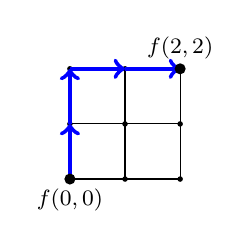
\begin{tikzpicture}
                \thegrid
                \draw[ultra thick, blue, ->] (0,0) -- (0,1);
                \draw[ultra thick, blue, ->] (0,1) -- (0,2);
                \draw[ultra thick, blue, ->] (0,2) -- (1,2);
                \draw[ultra thick, blue, ->] (1,2) -- (2,2);
                \fill[black]
                    (0,0) circle (2pt) node[below] {$f(0,0)$}
                    (2,2) circle (2pt) node[above] {$f(2,2)$};
            \end{tikzpicture}&
            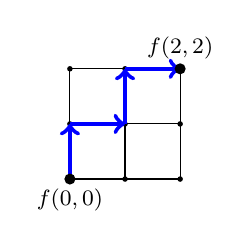
\begin{tikzpicture}
                \thegrid
                \draw[ultra thick, blue, ->] (0,0) -- (0,1);
                \draw[ultra thick, blue, ->] (0,1) -- (1,1);
                \draw[ultra thick, blue, ->] (1,1) -- (1,2);
                \draw[ultra thick, blue, ->] (1,2) -- (2,2);
                \fill[black]
                    (0,0) circle (2pt) node[below] {$f(0,0)$}
                    (2,2) circle (2pt) node[above] {$f(2,2)$};
            \end{tikzpicture}&
            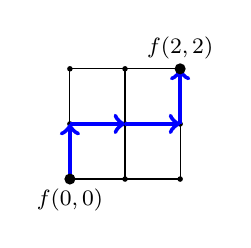
\begin{tikzpicture}
                \thegrid
                \draw[ultra thick, blue, ->] (0,0) -- (0,1);
                \draw[ultra thick, blue, ->] (0,1) -- (1,1);
                \draw[ultra thick, blue, ->] (1,1) -- (2,1);
                \draw[ultra thick, blue, ->] (2,1) -- (2,2);
                \fill[black]
                    (0,0) circle (2pt) node[below] {$f(0,0)$}
                    (2,2) circle (2pt) node[above] {$f(2,2)$};
            \end{tikzpicture}\\
            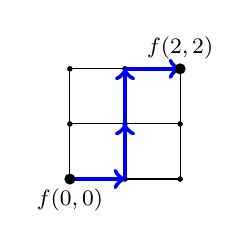
\begin{tikzpicture}
                \thegrid
                \draw[ultra thick, blue, ->] (0,0) -- (1,0);
                \draw[ultra thick, blue, ->] (1,0) -- (1,1);
                \draw[ultra thick, blue, ->] (1,1) -- (1,2);
                \draw[ultra thick, blue, ->] (1,2) -- (2,2);
                \fill[black]
                    (0,0) circle (2pt) node[below] {$f(0,0)$}
                    (2,2) circle (2pt) node[above] {$f(2,2)$};
            \end{tikzpicture}&
            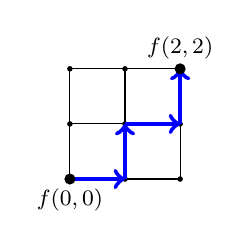
\begin{tikzpicture}
                \thegrid
                \draw[ultra thick, blue, ->] (0,0) -- (1,0);
                \draw[ultra thick, blue, ->] (1,0) -- (1,1);
                \draw[ultra thick, blue, ->] (1,1) -- (2,1);
                \draw[ultra thick, blue, ->] (2,1) -- (2,2);
                \fill[black]
                    (0,0) circle (2pt) node[below] {$f(0,0)$}
                    (2,2) circle (2pt) node[above] {$f(2,2)$};
            \end{tikzpicture}&
            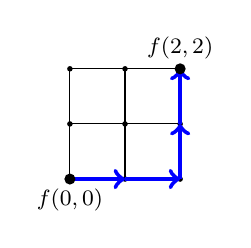
\begin{tikzpicture}
                \thegrid
                \draw[ultra thick, blue, ->] (0,0) -- (1,0);
                \draw[ultra thick, blue, ->] (1,0) -- (2,0);
                \draw[ultra thick, blue, ->] (2,0) -- (2,1);
                \draw[ultra thick, blue, ->] (2,1) -- (2,2);[]
                \fill[black]
                    (0,0) circle (2pt) node[below] {$f(0,0)$}
                    (2,2) circle (2pt) node[above] {$f(2,2)$};
            \end{tikzpicture}
        \end{tabular}
    \end{center}
    \caption{The six constraints on the computation of $f(2, 2)$.
%    $\shift 2 \shift 2 \shift 1 \shift 1 f = \shift 2 \shift 1 \shift 2 \shift 1 f = \shift 2 \shift 1 \shift 1 \shift 2 f = \shift 1 \shift 2 \shift 2 \shift 1 f = \shift 1 \shift 2 \shift 1 \shift 2 f = \shift 1 \shift 1 \shift 2 \shift 2 f$.
    }
    \label{fig:polyrec constraints}
\end{figure}

\paragraph{Multivariate \CDA~series}
%
In the second problem, we consider the notion of
\emph{constructible differentially algebraic} (\CDA) power series in commuting variables~\cite{BergeronReutenauer:EJC:1990}.
%
They were introduced in the multivariate context by Bergeron and Sattler~\cite{BergeronSattler:TCS:1995},
as solutions of systems of \emph{polynomial differential equations} of a restricted form (\cf~\cref{sec:CDA algebra} for details).
%
Such systems may not have solutions
and deciding whether this is the case is open~\cite[Remark 27]{Clemente:CONCUR:2024}.
%
Solvability of polynomial differential equations is undecidable
by a result of Denef and Lipshitz~\cite[Theorem 4.11]{DenefLipshitz:1984}
(\cref{rem:undecidability of solvability}),
and thus it is not clear whether \CDA~series have a decidable syntax.
%
We overcome this issue by showing that commutativity of shuffle automata
can be used to decide whether \CDA~systems are solvable~(\cref{thm:decidability of CDA solvability}),
thus answering the open question positively.

\subsection*{Organisation}
%
In the next section~\cref{sec:preliminaries} we present some preliminaries,
followed in~\cref{sec:commutativity} by a proof of~\cref{thm:commutativity for effective prevarieties}.
%
In \cref{sec:recognisable} we recall some known results about finite weighted automata,
which will help to put the following results in perspective.
%
Polynomial automata will be studied in~\cref{sec:Hadamard},
followed by shuffle automata in~\cref{sec:shuffle},
and infiltration automata in~\cref{sec:infiltration}.
%
(Thus the proof of \cref{thm:main theorem} is spread over these three sections.)
%
In the last section, an important remark shows that our techniques do not only solve the zeroness, equality, and commutativity problems,
but in fact we can construct a finite representation for the \emph{effective algebraic variety}
of all initial conditions ensuring zeroness, equality, resp., commutativity (\cref{rem:effective algebraic varieties}).
%
% In~\cref{sec:extensions} we discuss some extensions of our results.
% In~\cref{sec:mixed product} we discuss an extension of our results where Hadamard, shuffle, and infiltration products can co-exist in the same model.

This paper is an extended version of~\cite{Clemente:LICS:2025}.
%
In comparison to~\cite{Clemente:LICS:2025},
we have included more details and all interesting proofs.
%
Moreover, we provide the complete development for infiltration automata (\cref{sec:infiltration}),
which before was just sketched.
%
We have also introduced a new closure property,
namely closure under left anti-derivatives (\cref{sec:commutativity}),
which allows us to provide a very simple argument showing that the equality prolem
reduces back to the commutativity problem.
%
The preliminary section \cref{sec:recognisable} providing a gentle introduction in the linear case is also new.